\label{Appendix:pixels_overview}
\section{Radiation damages}
    Radiation hardness is a fundamental requirement for pixels detector especially in HEP since they are almost always installed near the interaction point where there is a high energy level of radiation. At LHC the $\phi_{eq}$ per year in the innermost pixel detector is $10^{14} n_{eq}/cm^2$; this number reduces by an order passing to the outer tracker layer \cite{K-Wermes} pag 341 Wermes. Here the high fluence of particles can cause a damage both in the substrate of the detector and in the superficial electronics. 
    
    The first one has a principal non ionizing nature, due to a non ionizing energy loss (NIEL), but it is related with the dislocation of the lattice caused by the collision with nuclei; by this fact the NIEL hypothesis states that the substrate damage is normalized to the damage caused by 1 MeV neutrons. Differently, surface damages are principally due to ionizing energy loss.

    \red{DUE PAROLE IN PIÙ SUL SURFACE DAMAGE}
    A charge accumulation in oxide ($S_iO_2$) can cause the generation of parasitic current with an obvious increase of the 1/f noise. Surface damages are mostly less relevant than the previous one, since with the development of microelectronics and with the miniaturization of components (in electronic industry 6-7 nm transistors are already used, while for MAPS the dimensions of components is around 180 nm) the quantity of oxide in circuit is reduced.

    Let's spend instead two more other words on the more-relevant substrate damages: the general result of high radiation level is the creation of new energy levels within the silicon band gap and depending on their energy-location their effect can be different, as described in the Shockely-Read-Hall (SRH) statistical model.
    \begin{figure}
        \centering
        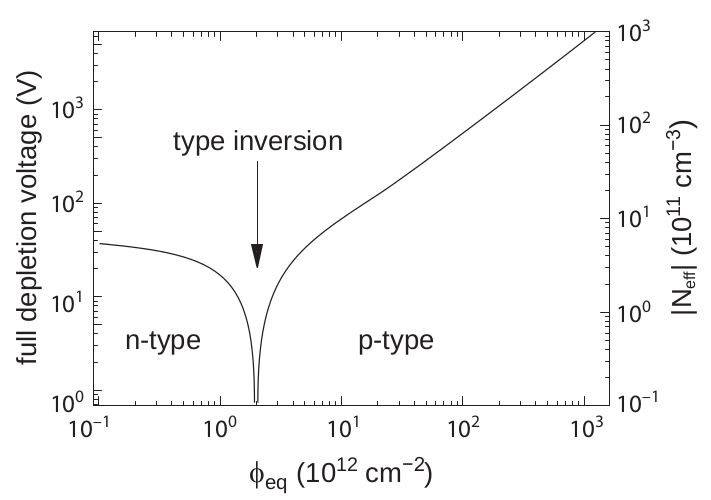
\includegraphics[width=.8\linewidth]{figures/overview/type_inversion.png}
        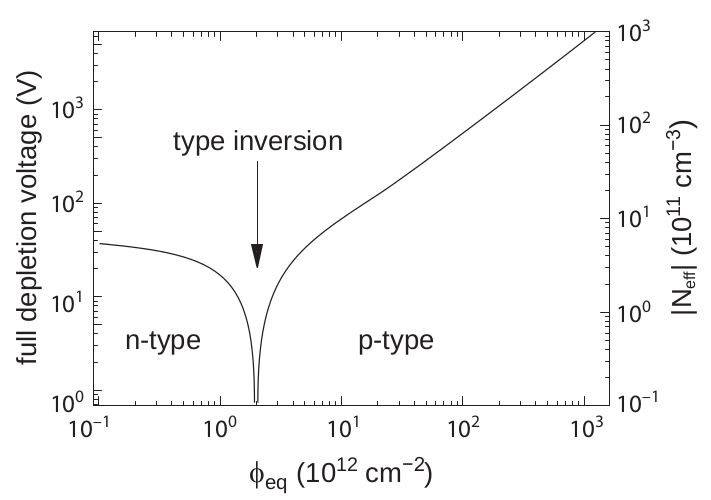
\includegraphics[width=.8\linewidth]{figures/overview/type_inversion.png}
        \caption{1b}
        \label{fig:type_inversion}
    \end{figure}
    The three main consequence of radiation damages are the changing of the effect doping concentration, the leakage current and the increasing of trapping probability.

    \textbf{Changing of the effective doping concentration:} is associated with the creation/removal of donors and acceptors center which trap respectively electrons/holes from the conduction band and cause a change in effective space charge density. Even an inversion (p-type becomes n-type\footnote{L'INVERSIONE OPPOSTA NON CE L'HAI PERCHÈ?}) can happen: indeed it is quite common at not too high fluences ($\phi_{eq} 10^{12-13}n_{eq}cm^{-2}$). 
    A changing in the doping concentration requires an adjustment of the biasing of the sensor during its lifetime (eq.\ref{eq:deplation_d}) and sometimes can be difficult keeping to fully deplete the bulk.

    \textbf{Leakage current:} is associated with the generation-recombination centers. It has a strong dependence with the temperature ($I_{leak}\propto T^2$), whose solution is therefore to operate at lower temperature.

    \textbf{Increase of trapping probability:} since the trapping probability is constant in the depleted region, the collected charge decreases exponentially with the drift path. The exponential coefficient, that is the mean trapping path, decreases after irradiation and typical values are 125-250 $\mu m$ and must be compared with the thickness of the depleted region which () corresponds to the mean drift path.

    Different choices for substrate resistivity, for junctions type and for detector design are typically made to fight radiation issues. Some material with high oxygen concentration (as crystal produced using Czochralki (Cz) or float-zone (Fz) process (\red{CONTROLLA LA DIFFERENZA TRA I DUE})) for example, show a compensation effect for radiation damage; another example is the usage of n+ -in-p/n sensors (even if p+ -in-n sensors are easier and cheaper to obtain) to get advantage of inversion/to have not the inversion (since they are already p-type). After inversion the n+p boundary, coming from n+ in-n, but to keep using the sensor the depletion zone still must be placed near the diode.
    
    \red{Single Event Upset, in sostanza è quando un bit ti cambia valore (da 0 a 1 o viceversa) perché una particella deposita carica nell'elettronica che fa da memoria registro/RAM/.... Questo tipo di elettronica ha bisogno di un sacco di carica prima che il bit si "flippi" (cambi valore), infatti tipicamente per avere un SEU non basta una MIP che attraversa esattemente quel pezzo di chip in cui è implementata la memoria, ma un adrone che faccia interazione nucleare producendo più carica di quanto farebbe una MIP. Questo metodo pur essendo più comodo richieda less amount of area ha però come drawback che il registro può essere soggetto a SEU problema non trascurabile in acceleratori come HL-LHC adronici}